

\documentclass[man,floatsintext]{apa6}
\usepackage{lmodern}
\usepackage{amssymb,amsmath}
\usepackage{ifxetex,ifluatex}
\usepackage{fixltx2e} % provides \textsubscript
\ifnum 0\ifxetex 1\fi\ifluatex 1\fi=0 % if pdftex
  \usepackage[T1]{fontenc}
  \usepackage[utf8]{inputenc}
\else % if luatex or xelatex
  \ifxetex
    \usepackage{mathspec}
  \else
    \usepackage{fontspec}
  \fi
  \defaultfontfeatures{Ligatures=TeX,Scale=MatchLowercase}
\fi
% use upquote if available, for straight quotes in verbatim environments
\IfFileExists{upquote.sty}{\usepackage{upquote}}{}
% use microtype if available
\IfFileExists{microtype.sty}{%
\usepackage{microtype}
\UseMicrotypeSet[protrusion]{basicmath} % disable protrusion for tt fonts
}{}
\usepackage{hyperref}
\hypersetup{unicode=true,
            pdftitle={GenSamp: RESULTS},
            pdfauthor={Gleb Furman~\& James E. Pustejovsky},
            pdfborder={0 0 0},
            breaklinks=true}
\urlstyle{same}  % don't use monospace font for urls
\usepackage{graphicx,grffile}
\makeatletter
\def\maxwidth{\ifdim\Gin@nat@width>\linewidth\linewidth\else\Gin@nat@width\fi}
\def\maxheight{\ifdim\Gin@nat@height>\textheight\textheight\else\Gin@nat@height\fi}
\makeatother
% Scale images if necessary, so that they will not overflow the page
% margins by default, and it is still possible to overwrite the defaults
% using explicit options in \includegraphics[width, height, ...]{}
\setkeys{Gin}{width=\maxwidth,height=\maxheight,keepaspectratio}
\IfFileExists{parskip.sty}{%
\usepackage{parskip}
}{% else
\setlength{\parindent}{0pt}
\setlength{\parskip}{6pt plus 2pt minus 1pt}
}
\setlength{\emergencystretch}{3em}  % prevent overfull lines
\providecommand{\tightlist}{%
  \setlength{\itemsep}{0pt}\setlength{\parskip}{0pt}}
\setcounter{secnumdepth}{0}
% Redefines (sub)paragraphs to behave more like sections
\ifx\paragraph\undefined\else
\let\oldparagraph\paragraph
\renewcommand{\paragraph}[1]{\oldparagraph{#1}\mbox{}}
\fi
\ifx\subparagraph\undefined\else
\let\oldsubparagraph\subparagraph
\renewcommand{\subparagraph}[1]{\oldsubparagraph{#1}\mbox{}}
\fi

%%% Use protect on footnotes to avoid problems with footnotes in titles
\let\rmarkdownfootnote\footnote%
\def\footnote{\protect\rmarkdownfootnote}


  \title{GenSamp: RESULTS}
    \author{Gleb Furman\textsuperscript{1}~\& James E. Pustejovsky\textsuperscript{1}}
    \date{}
  
\shorttitle{RESULTS}
\affiliation{
\vspace{0.5cm}
\textsuperscript{1} University of Texas at Austin}
\usepackage{csquotes}
\usepackage{upgreek}
\captionsetup{font=singlespacing,justification=justified}

\usepackage{longtable}
\usepackage{lscape}
\usepackage{multirow}
\usepackage{tabularx}
\usepackage[flushleft]{threeparttable}
\usepackage{threeparttablex}

\newenvironment{lltable}{\begin{landscape}\begin{center}\begin{ThreePartTable}}{\end{ThreePartTable}\end{center}\end{landscape}}

\makeatletter
\newcommand\LastLTentrywidth{1em}
\newlength\longtablewidth
\setlength{\longtablewidth}{1in}
\newcommand{\getlongtablewidth}{\begingroup \ifcsname LT@\roman{LT@tables}\endcsname \global\longtablewidth=0pt \renewcommand{\LT@entry}[2]{\global\advance\longtablewidth by ##2\relax\gdef\LastLTentrywidth{##2}}\@nameuse{LT@\roman{LT@tables}} \fi \endgroup}

\begin{document}
\maketitle

\hypertarget{methods-summary}{%
\section{Methods Summary}\label{methods-summary}}

\hypertarget{clustering}{%
\subsection{Clustering}\label{clustering}}

\begin{verbatim}
## Warning: package 'tableone' was built under R version 3.5.3
\end{verbatim}

\begin{table}[H]
\centering
\begin{tabular}{l|l|l}
\hline
strata & var & SMD\\
\hline
1 & dSCH & 0.11\\
\hline
1 & ethBlack & \textbackslash{}textbf\{-0.39\}\\
\hline
1 & ethHisp & -0.22\\
\hline
1 & ethWhite & \textbackslash{}textbf\{0.47\}\\
\hline
1 & n & 0.01\\
\hline
1 & pELL & 0.02\\
\hline
1 & pFem & 0\\
\hline
1 & pTotfrl & \textbackslash{}textbf\{-0.49\}\\
\hline
1 & ST.ratio & 0.03\\
\hline
1 & Suburban & \textbackslash{}textbf\{0.83\}\\
\hline
1 & T1 & \textbackslash{}textbf\{-0.71\}\\
\hline
1 & ToRu & -0.02\\
\hline
1 & Urban & \textbackslash{}textbf\{-0.81\}\\
\hline
2 & dSCH & \textbackslash{}textbf\{0.33\}\\
\hline
2 & ethBlack & -0.19\\
\hline
2 & ethHisp & \textbackslash{}textbf\{0.71\}\\
\hline
2 & ethWhite & \textbackslash{}textbf\{-0.77\}\\
\hline
2 & n & \textbackslash{}textbf\{0.46\}\\
\hline
2 & pELL & \textbackslash{}textbf\{0.68\}\\
\hline
2 & pFem & 0.06\\
\hline
2 & pTotfrl & 0.05\\
\hline
2 & ST.ratio & \textbackslash{}textbf\{0.52\}\\
\hline
2 & Suburban & 0.12\\
\hline
2 & T1 & \textbackslash{}textbf\{-0.61\}\\
\hline
2 & ToRu & \textbackslash{}textbf\{-0.99\}\\
\hline
2 & Urban & \textbackslash{}textbf\{0.67\}\\
\hline
3 & dSCH & \textbackslash{}textbf\{-0.89\}\\
\hline
3 & ethBlack & -0.03\\
\hline
3 & ethHisp & \textbackslash{}textbf\{-1.15\}\\
\hline
3 & ethWhite & \textbackslash{}textbf\{1.03\}\\
\hline
3 & n & -0.23\\
\hline
3 & pELL & \textbackslash{}textbf\{-1.15\}\\
\hline
3 & pFem & -0.05\\
\hline
3 & pTotfrl & \textbackslash{}textbf\{-1.04\}\\
\hline
3 & ST.ratio & -0.09\\
\hline
3 & Suburban & \textbackslash{}textbf\{0.76\}\\
\hline
3 & T1 & \textbackslash{}textbf\{-0.75\}\\
\hline
3 & ToRu & 0.25\\
\hline
3 & Urban & \textbackslash{}textbf\{-0.96\}\\
\hline
4 & dSCH & \textbackslash{}textbf\{0.3\}\\
\hline
4 & ethBlack & \textbackslash{}textbf\{0.27\}\\
\hline
4 & ethHisp & \textbackslash{}textbf\{0.87\}\\
\hline
4 & ethWhite & \textbackslash{}textbf\{-0.98\}\\
\hline
4 & n & 0.05\\
\hline
4 & pELL & \textbackslash{}textbf\{0.76\}\\
\hline
4 & pFem & 0.02\\
\hline
4 & pTotfrl & \textbackslash{}textbf\{1.1\}\\
\hline
4 & ST.ratio & 0.1\\
\hline
4 & Suburban & \textbackslash{}textbf\{-0.72\}\\
\hline
4 & T1 & \textbackslash{}textbf\{1.31\}\\
\hline
4 & ToRu & -0.13\\
\hline
4 & Urban & \textbackslash{}textbf\{0.82\}\\
\hline
5 & dSCH & -0.1\\
\hline
5 & ethBlack & 0.17\\
\hline
5 & ethHisp & \textbackslash{}textbf\{0.69\}\\
\hline
5 & ethWhite & \textbackslash{}textbf\{-0.43\}\\
\hline
5 & n & -0.08\\
\hline
5 & pELL & \textbackslash{}textbf\{0.54\}\\
\hline
5 & pFem & -0.05\\
\hline
5 & pTotfrl & \textbackslash{}textbf\{1.08\}\\
\hline
5 & ST.ratio & \textbackslash{}textbf\{-0.29\}\\
\hline
5 & Suburban & \textbackslash{}textbf\{0.83\}\\
\hline
5 & T1 & \textbackslash{}textbf\{1.31\}\\
\hline
5 & ToRu & \textbackslash{}textbf\{0.48\}\\
\hline
5 & Urban & \textbackslash{}textbf\{-1.21\}\\
\hline
6 & dSCH & 0.24\\
\hline
6 & ethBlack & 0.07\\
\hline
6 & ethHisp & \textbackslash{}textbf\{-0.82\}\\
\hline
6 & ethWhite & \textbackslash{}textbf\{0.76\}\\
\hline
6 & n & -0.17\\
\hline
6 & pELL & \textbackslash{}textbf\{-0.77\}\\
\hline
6 & pFem & 0.01\\
\hline
6 & pTotfrl & \textbackslash{}textbf\{-0.71\}\\
\hline
6 & ST.ratio & \textbackslash{}textbf\{-0.35\}\\
\hline
6 & Suburban & \textbackslash{}textbf\{-1.21\}\\
\hline
6 & T1 & \textbackslash{}textbf\{-0.71\}\\
\hline
6 & ToRu & \textbackslash{}textbf\{0.49\}\\
\hline
6 & Urban & \textbackslash{}textbf\{0.82\}\\
\hline
\end{tabular}
\end{table}

\hypertarget{participation-generating-model}{%
\subsection{Participation Generating Model}\label{participation-generating-model}}

\begin{table}[H]
\centering
\begin{tabular}{l|l|r}
\hline
Variables & vnames & log\_odds\\
\hline
Schoolwide Title I & T1 & 0.019\\
\hline
Total Students & n & 0.374\\
\hline
\% FRL & pTotfrl & 0.081\\
\hline
Urban & Urban & 0.433\\
\hline
Suburban & Suburban & 0.007\\
\hline
Town/Rural & ToRu & -0.403\\
\hline
\% White & ethWhite & -0.538\\
\hline
\% Black & ethBlack & 0.291\\
\hline
\% Hispanic & ethHisp & 0.395\\
\hline
\% Female & pFem & -0.019\\
\hline
Student/Teacher Ratio & ST.ratio & -0.101\\
\hline
Total District Schools & dSCH & 0.520\\
\hline
\% ELL & pELL & 0.412\\
\hline
\end{tabular}
\end{table}

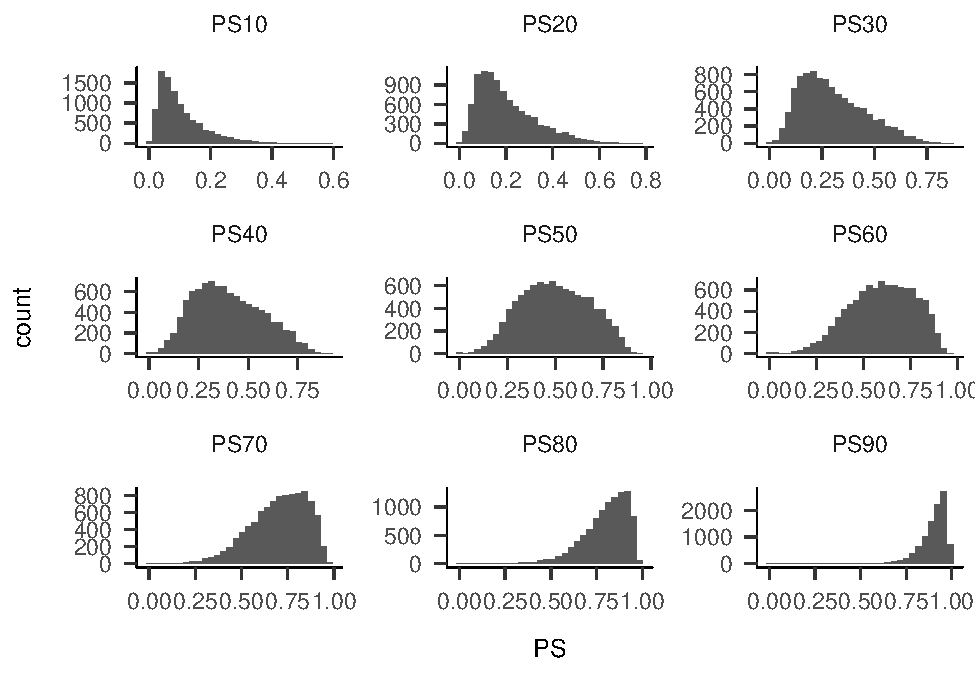
\includegraphics{Results_files/figure-latex/unnamed-chunk-4-1.pdf}

\begin{figure}
\centering
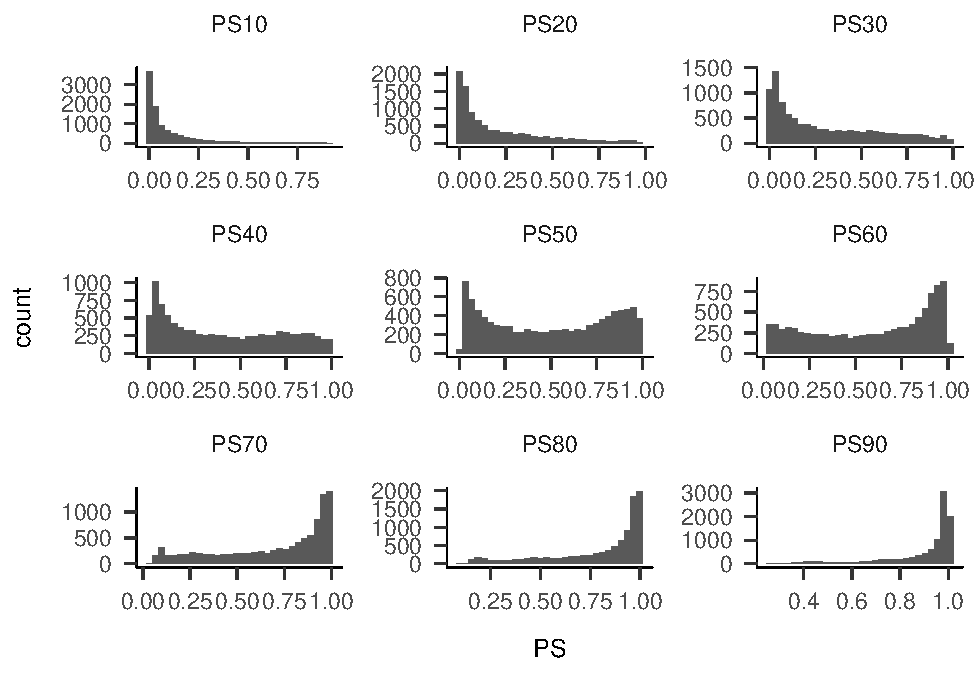
\includegraphics{Results_files/figure-latex/unnamed-chunk-5-1.pdf}
\caption{\label{fig:unnamed-chunk-5}Distributions of Participation Propensity Scores}
\end{figure}

\hypertarget{b-index}{%
\subsection{B Index}\label{b-index}}

\begin{figure}
\centering
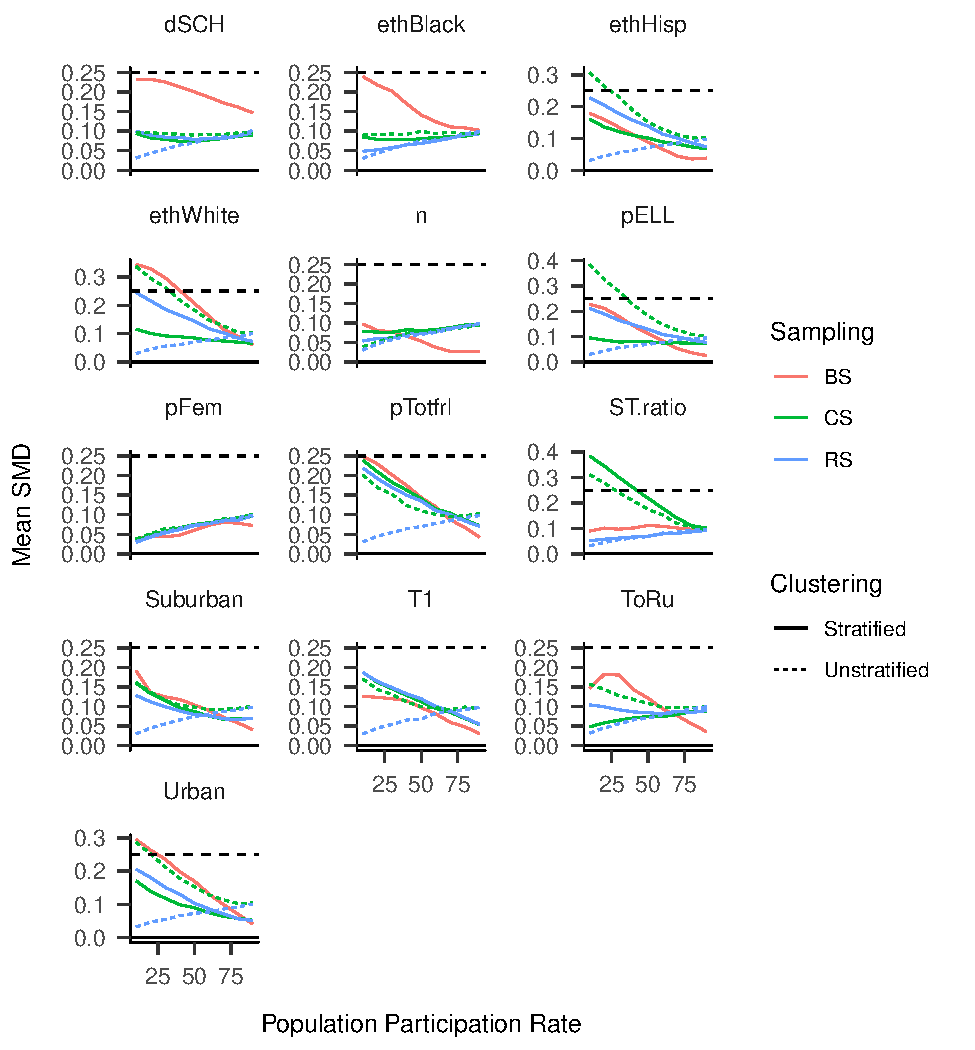
\includegraphics{Results_files/figure-latex/unnamed-chunk-8-1.pdf}
\caption{\label{fig:unnamed-chunk-8}Averge B-Index}
\end{figure}

\begin{verbatim}
## # A tibble: 5 x 13
## # Groups:   sample, Clustering, Sampling [5]
##   sample Clustering Sampling     K  `10`  `20`  `30`  `40`  `50`  `60`
##   <chr>  <chr>      <chr>    <dbl> <int> <int> <int> <int> <int> <int>
## 1 S_BS   Stratified BS           6     0     0     0     0     0     0
## 2 S_CS   Stratified CS           6     0     7     4     4     0     0
## 3 S_RS   Stratified RS           6     0     0     0     0     0     0
## 4 U_CS   Unstratif~ CS          NA     6     4     5     1     3     0
## 5 U_RS   Unstratif~ RS          NA     2     3     2     0     1     0
## # ... with 3 more variables: `70` <int>, `80` <int>, `90` <int>
\end{verbatim}

\hypertarget{standardized-mean-differences}{%
\subsection{Standardized mean differences}\label{standardized-mean-differences}}

\begin{figure}
\centering
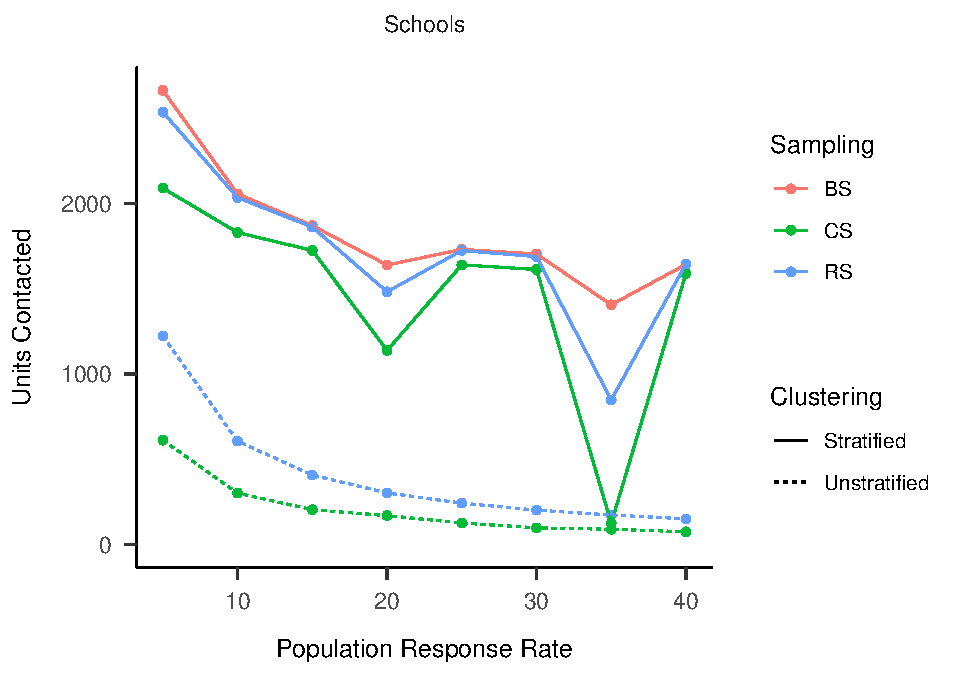
\includegraphics{Results_files/figure-latex/unnamed-chunk-9-1.pdf}
\caption{\label{fig:unnamed-chunk-9}Average SMDs}
\end{figure}

\hypertarget{sampling-difficulty}{%
\subsection{Sampling Difficulty}\label{sampling-difficulty}}

\begin{figure}
\centering
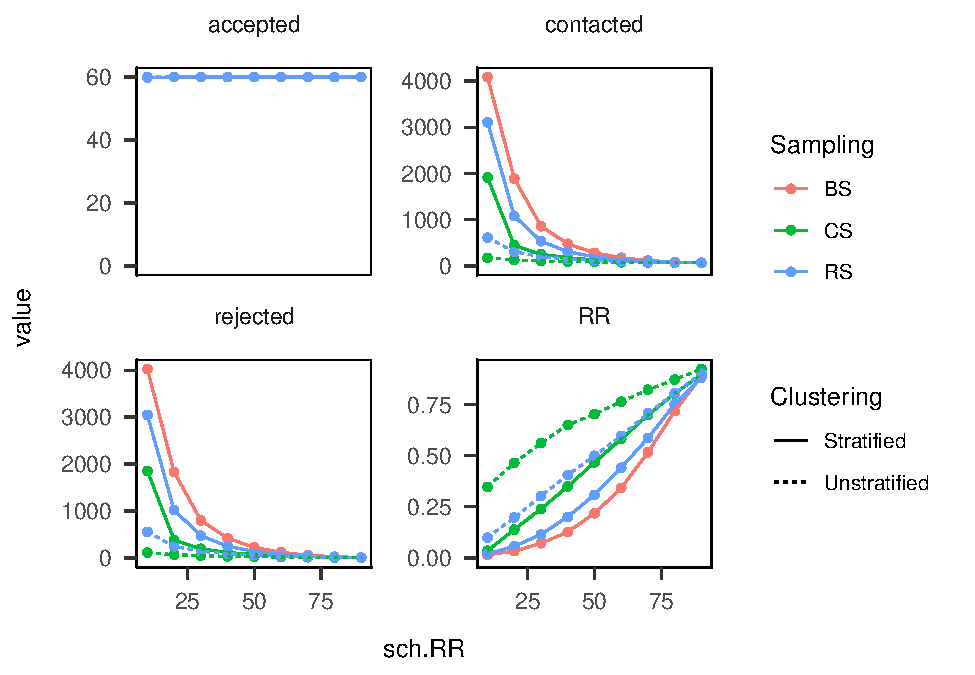
\includegraphics{Results_files/figure-latex/unnamed-chunk-11-1.pdf}
\caption{\label{fig:unnamed-chunk-11}Recruitment Counts}
\end{figure}

\begin{figure}
\centering
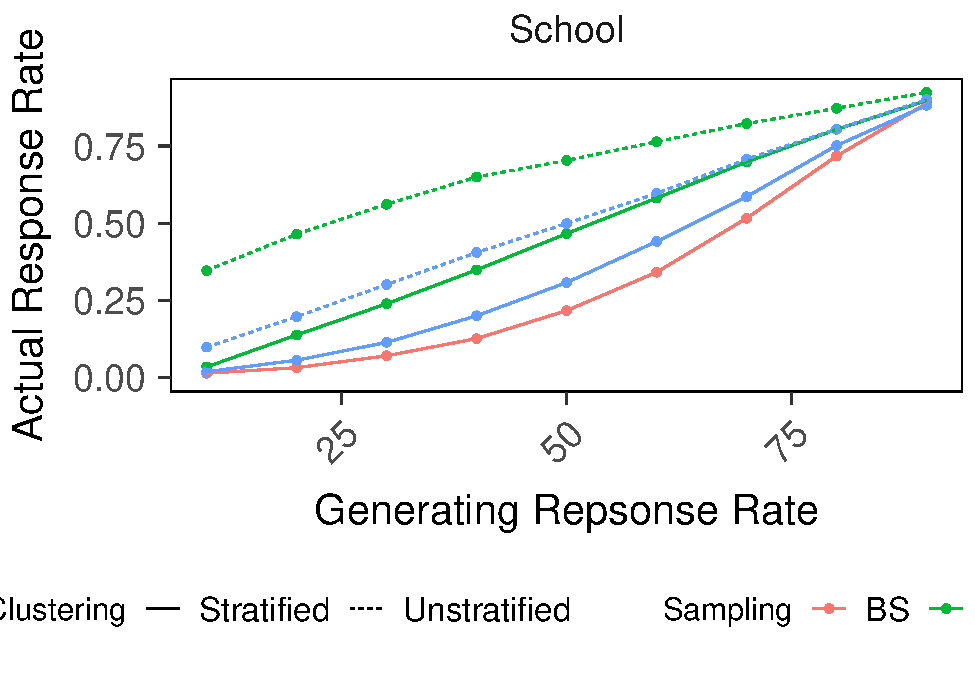
\includegraphics{Results_files/figure-latex/unnamed-chunk-13-1.pdf}
\caption{\label{fig:unnamed-chunk-13}Sampling response rates}
\end{figure}


\end{document}
